% This is a LaTeX template
% for preparing documents for ITTMM conference

\documentclass[60x84/16,8pt]{ittmm}

% Убедительная просьба к авторам не редактировать файл definition.tex
\usepackage[T1,T2A]{fontenc}
\usepackage{ucs}
\usepackage[utf8x]{inputenc}
\usepackage[english,russian]{babel}

%% Расширенная математика

\usepackage{amsmath}
\usepackage{amssymb}
\usepackage{amscd}

\usepackage{mathtools}
\mathtoolsset{
showonlyrefs=true,
mathic=true,
}

\allowdisplaybreaks

%% Работа с графикой

\usepackage{graphicx}

%% hyperref

\usepackage{hyperref}
\hypersetup{backref,
 colorlinks=false}
\hypersetup{pdfborder=0 0 0}

%% local definitions

\geometry{twoside}
\geometry{bindingoffset=0pt}

\geometry{includehead}
\geometry{hmargin={16mm,16mm},vmargin={12mm,13mm}}
\geometry{marginparwidth=0pt,marginparsep=0pt}
\geometry{headheight=0pt}
\geometry{headsep=\baselineskip}

\pagestyle{empty}

\usepackage{cite}


\begin{document}

% Укажите индекс УДК, соответствующий Вашей работе.
\udc{519.25}

\title{Разработка эффективного алгоритма краткосрочного прогнозирования электропотребления с использованием ансамблирования}

\author[1]{Е. Ю. Щетинин}
\author[2]{М. В. Бережков}
\author[2]{П. Г. Любин}

\address[1]{Всероссийский научно-исследовательский институт\\
  по проблемам гражданской обороны  и чрезвычайных ситуаций\\
  МЧС России (федеральный центр науки и высоких технологий)\\
  ул. Давыдковская, д.7, Москва, Россия, 121352}
\address[2]{Федеральное государственное бюджетное образовательное учреждение\\
  Высшего образования\\
  Московский государственный технологический университет ``СТАНКИН''\\
  пер. Вадковский, д.3а, Москва, Россия, 127055}

\email{\url{lyubin.p@gmail.com}, \url{riviera-molto@mail.ru}}

\begin{abstract}
Краткосрочное прогнозирование потребления электроэнергии является актуальной
задачей во многих областях в виду специфичности продукта: нельзя накопить и
хранить энергию впрок. Во-первых, предприятиям-участникам оптового рынка
электроэнергии необходимо заранее подавать заявки с плановым потреблением, а
энергогенерирующим предприятиям необходимо планировать мощности. Во-вторых,
подобный показатель может использоваться при построение других моделей в
качестве признака. При этом потребление электрической энергии каким-либо
объектом (цехом, промышленным предприятием, энергообъединением и т.п.) является
временным рядом, так как представляет собой мгновенные значения потребляемой
мощности замеренные в различные моменты времени с определенной периодичностью. В
данной работе продемонстрирован простой и эффективный метод краткосрочного
прогнозирования электропотребления. Метод основывается на ансамблировании
базовых моделей (RPART - Recursive PARTitioning, CTREE - Conditional Inference
Trees) и имеет хороший уровень прогнозирования, который сопоставим с более
сложными в использовании алгоритмами. Ансамблирование представляет собой
алгоритм комбинации набора обученных моделей с целью повышения точности
прогноза, при этом стараясь избежать переобучения. Существует несколько методов
ансамблирования, которые имеют свои недостатки и преимущества. В данной работе
мы использовали метод бэггинга (Bagging = Bootstrap aggregating), который помог
улучшить прогностическую силу отдельных базовых моделей.
\end{abstract}

\keywords{краткосрочное прогнозирование, ансамблирование, RPART, CTREE, случайные деревья, электропотребление, бэггинг}

% https://www.google.ru/search?q=%D0%B0%D0%BD%D1%81%D0%B0%D0%BC%D0%B1%D0%BB%D0%B8%% D0%BE%D1%80%D0%BE%D0%B2%D0%B0%D0%BD%D0%B8%D0%B5&oq=%D0%B0%D0%BD%D1%81%D0%B0%D0%B% C%D0%B1%D0%BB%D0%B8%D0%BE%D1%80%D0%BE%D0%B2%D0%B0%D0%BD%D0%B8%D0%B5&aqs=chrome..% 69i57j0l5.9853j0j7&sourceid=chrome&ie=UTF-8

% https://alexanderdyakonov.wordpress.com/2017/03/10/c%D1%82%D0%B5%D0%BA%D0%B8%D0%% BD%D0%B3-stacking-%D0%B8-%D0%B1%D0%BB%D0%B5%D0%BD%D0%B4%D0%B8%D0%BD%D0%B3-blendi% ng

% http://www.machinelearning.ru/wiki/images/5/56/Guschin2015Stacking.pdf

% \thanks{Рукопись должна содержать УДК, который рекомендуется брать из
%   следующего источника: \url{http://www.mathnet.ru/udc.pdf}.}

\alttitle{Development of an effective algorithm for short-term forecasting of power consumption using ensemble}

\altauthor[1]{E. Yu. Shchetinin}
\altauthor[2]{M. V. Berezhkov}
\altauthor[2]{P. G. Lyubin}

\altaddress[1]{All-Russian Research Institute\\
  for Civil Defense and Emergencies of the MER\\
  (Science and High Technology Federal Center)\\
  Davydkovskaya str., 7, Moscow, 121352, Russia}
\altaddress[2]{Moscow State University of Technology ``STANKIN'',\\ 
  Vadkovsky lane, 3a, Moscow, 127055, Russia}

\begin{altabstract}
Place here short abstract in English (between 150 and 250 words).
\end{altabstract}

\altkeywords{short-term forecast, ensemble, RPART, CTREE, random trees, power consumption, bagging}

\maketitle

\section{Введение}
\label{sec:intro}
К наиболее распространенным методам прогнозирования временных рядов относятся \cite{Tihonov2006}:
\begin{itemize}
    \item прогнозная экстраполяция
    \item экспертные (интуитивные) методы прогнозирования
    \item корреляционный и регрессионный анализы
    \item прогнозирование на базе ARIMA моделей
    \item адаптивные методы прогнозирования
    \item прогнозирование с использованием искусственных нейронных сетей
    \item прогнозирование с использованием гибридных сетей
\end{itemize}

Перечисленные методы могут применяться для прогнозирования электропотребления и
обладают присущими им достоинствами и недостатками, подробно описанными в
\cite{Tihonov2006}. В современных работах чаще остальных описываются решения
данной задачи с применением искусственных нейронных сетей, к недостаткам которых
можно отнести сложность настройки и сложность интерпретации. В данной работе мы
используем подход, в котором используется ансамбль методов.

На рисунке ниже изображена динамика почасового потребления электроэнергии в
России за 3 недели 2017 года: с 13 июня по 3 июля.
\begin{figure}
  \centering
  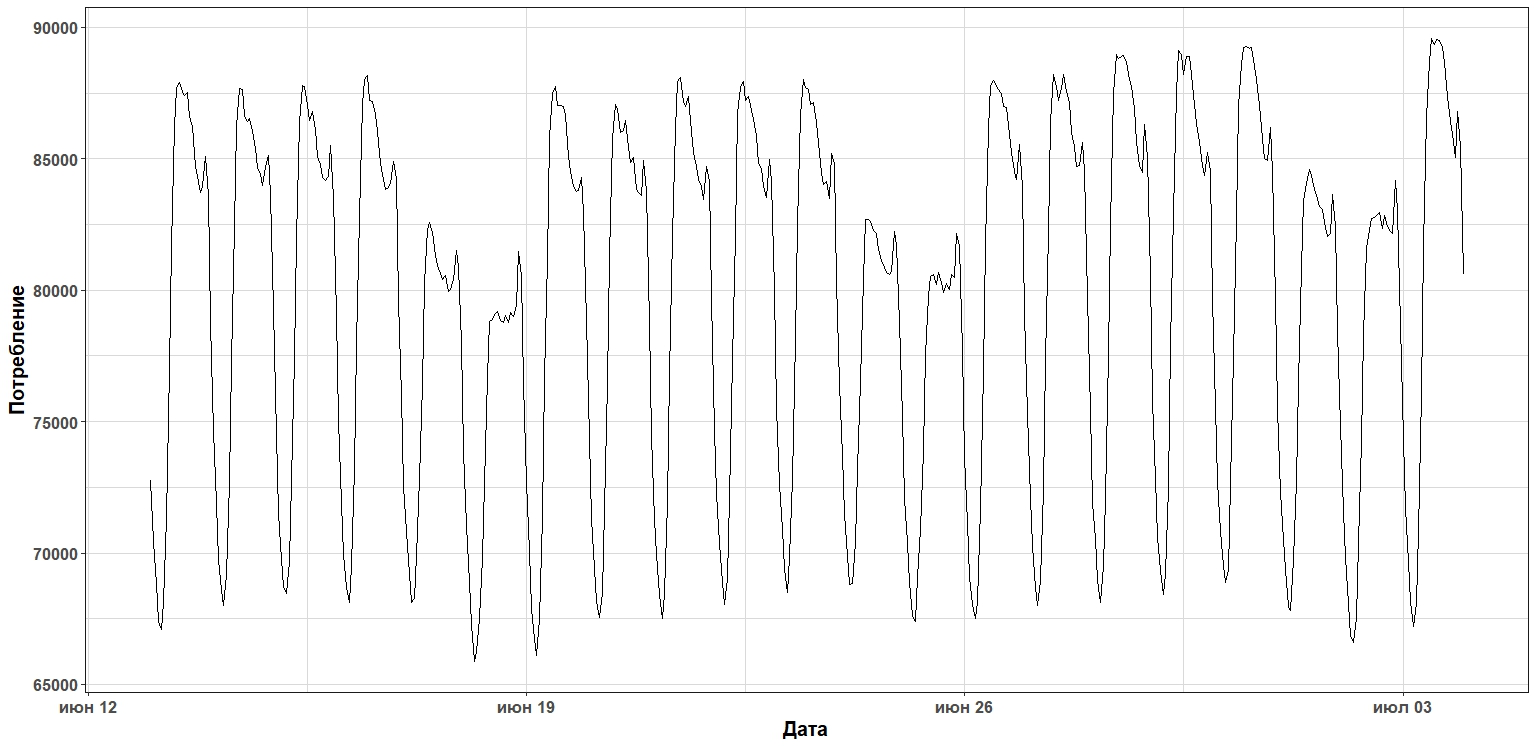
\includegraphics[width=0.8\linewidth]{Ru/train_dataset.jpeg}
  \caption{Исходные данные}
  \label{fig:data}
\end{figure}

\section{Метод}
\label{sec:methods}
К наиболее распространенным методам ансамблирования относятся \cite{Tihonov2006}:
\begin{itemize}
    \item простое голосование (Simple Voting)
    \item взвешенное голосование (Weighted Voting)
    \item смесь экспертов (Mixture of Experts [19])
    \item бустинг (Boosting)
    \item бэггинг (Bagging = Bootstrap aggregating)
\end{itemize}
В своей работе мы использовали бэггинг, который был предложен Л. Брейманом в
1996 году [4]. Суть метода заключается в формировании различных обучающих
подвыборок случайным выбором с возвращениями - некоторые объекты попадают в
подвыборку несколько раз, некоторые ни разу. Базовые алгоритмы, обученные по
подвыборкам, объединяются в композицию с помощью простого голосования.
Достоинствами бэггинга являются: во-первых, возможность использования различных
базовых алгоритмов, ошибки которых могут быть взаимно компенсированы при
голосовании; во-вторых, некоторые обучающие подвыборки могут не содержать
объекты-выбросы и алгоритм, построенный по этим подвыборкам, может оказаться
точнее алгоритма, построенного по полной выборке. В данной работе в качестве
базовых алгоритмов используются RPART и CTREE. Результат прогнозирования
потребления электроэнергии на одни сутки вперед приведен на рисунке ниже.
\begin{figure}
  \centering
  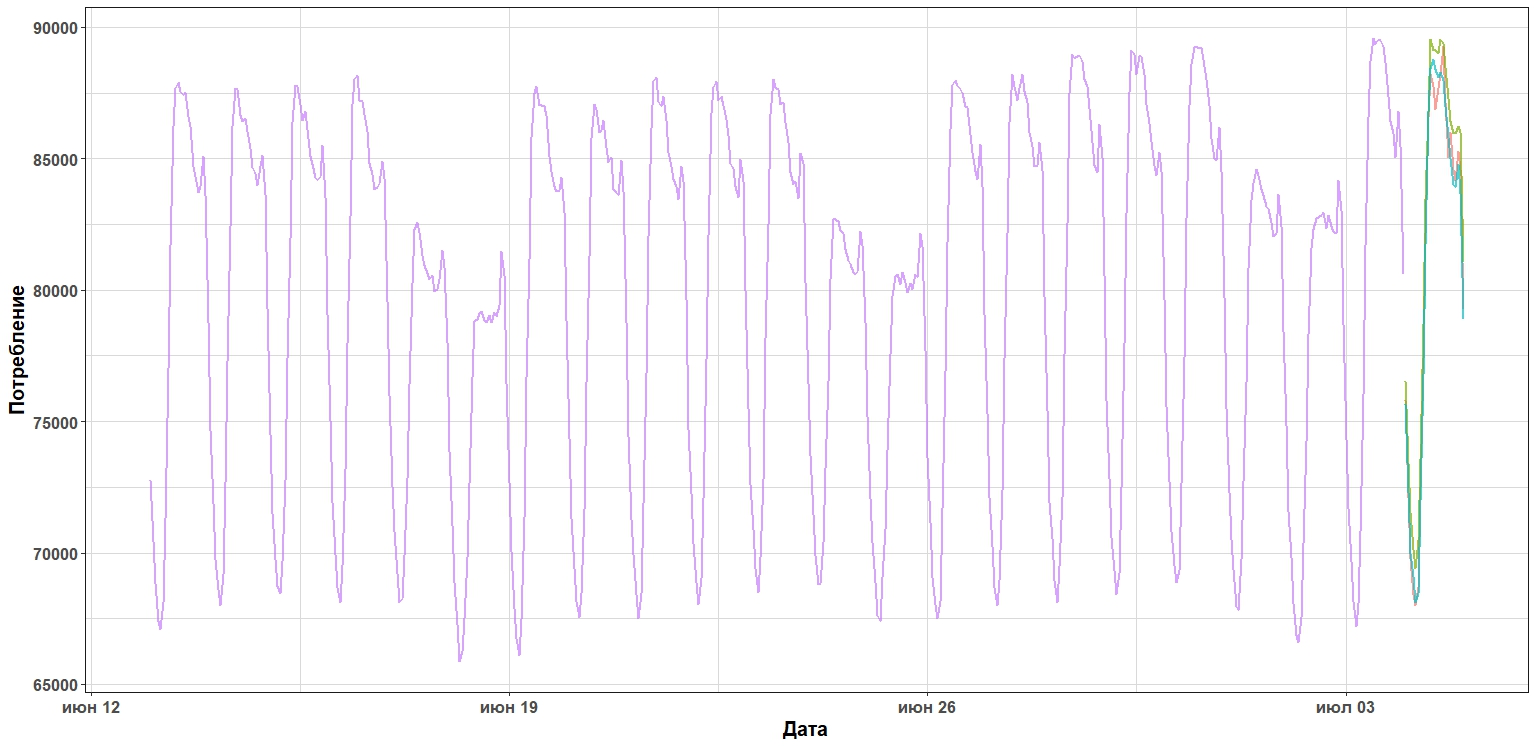
\includegraphics[width=0.8\linewidth]{Ru/prediction.jpeg}
  \caption{Прогноз}
  \label{fig:prediction}
\end{figure}


\section{Заключение}
В данной работе продемонстрирован простой и эффективный метод краткосрочного
прогнозирования электропотребления, который может использоваться участниками
рынка энергии при планировании генерации и при планировании закупок.

\begin{thebibliography}{99}

\bibitem{Shetinin}
Е.~Ю. Щетинин, Эффективные компьютерные алгоритмы моделирования спотовых цен на
электроэнергию. - Научное обозрение, 2016. №22, 237-242 с.

\bibitem{ShetininKaplunovMarkov}
Е.~Ю. Щетинин, С.~В. Каплунов, П.~Н. Марков, Моделирование спотовых цен на
электроэнергию с использованием марковских процессов переключения режимов. -
Вестник РУДН, Серия Математика. Информатика. Физика, 2012, №3, 61-68 с.

\bibitem{ShetininLyubin}
Е.~Ю. Щетинин, П.~Г. Любин, Робастный алгоритм построения сглаживающих сплайнов.
- Научное Обозрение, 2015. №1, 86–94 с.

\bibitem{LyubinShetinin}
П.~Г. Любин, Е.~Ю. Щетинин, Стохастические модели сглаживания и прогнозирования
коэффициентов смертности. - Научное Обозрение, 2015, №18, 147–155 с.

\bibitem{Breiman}
L. Breiman, J.~H. Friedman, R.~A. Olshen, C.~J. Stone, Classification and
Regression Trees. - Wadsworth, California.

\end{thebibliography}


% % Возможно использовать bibtex.
% \bibliographystyle{elsarticle-num}
% \bibliography{ittmm-template-ru}


\makealttitle      

\end{document}
